% !TEX root = ../thesis.tex
\chapter{Approach}

% **************************** Define Graphics Path **************************
\ifpdf
    \graphicspath{{Chapter3/Figs/Raster/}{Chapter3/Figs/PDF/}{Chapter3/Figs/}}
\else
    \graphicspath{{Chapter3/Figs/Vector/}{Chapter3/Figs/}}
\fi

\section{Introduction}

Despite the importance of crowd monitoring in mass gathering events, the literature review in the previous chapter is able to identify several gaps in the research, especially in crowd modelling. Most state-of-art crowd monitoring techniques do not incorporate a typology to distinguish different types of crowd. In other words, no explicit type of crowd is defined in those approaches.

say something more about crowd modelling

conclude with the need of a crowd monitoring framework

\section[Overview of the Mobile Crowd Monitoring for Emergency Management in Mass Gathering]{\texorpdfstring{Overview of the Mobile Crowd Monitoring for \\Emergency Management in Mass Gathering}}

In this project, we propose the crowd monitoring framework for emergency management in mass gatherings. The objectives of the framework are: 
\begin{inparaenum}[i)]
	\item to incorporate more sources of contextual data;
	\item to classify a crowd into different crowd types;
	\item to propose a set of crowd attributes and describe a crowd type under those attributes
\end{inparaenum}.

To achieve those objectives, as can be seen in Figure \ref{fig:frameworkOverview} the framework consists of three layers:
\begin{inparaenum}[i)]
	\item Context data to handle different sources of information;
	\item Crowd model to analyse the context data and classify type of a crowd;
	\item Crowd monitoring to detect the dangerous crowd types in real time
\end{inparaenum}.

\begin{figure}[htbp!] 
	\centering    
	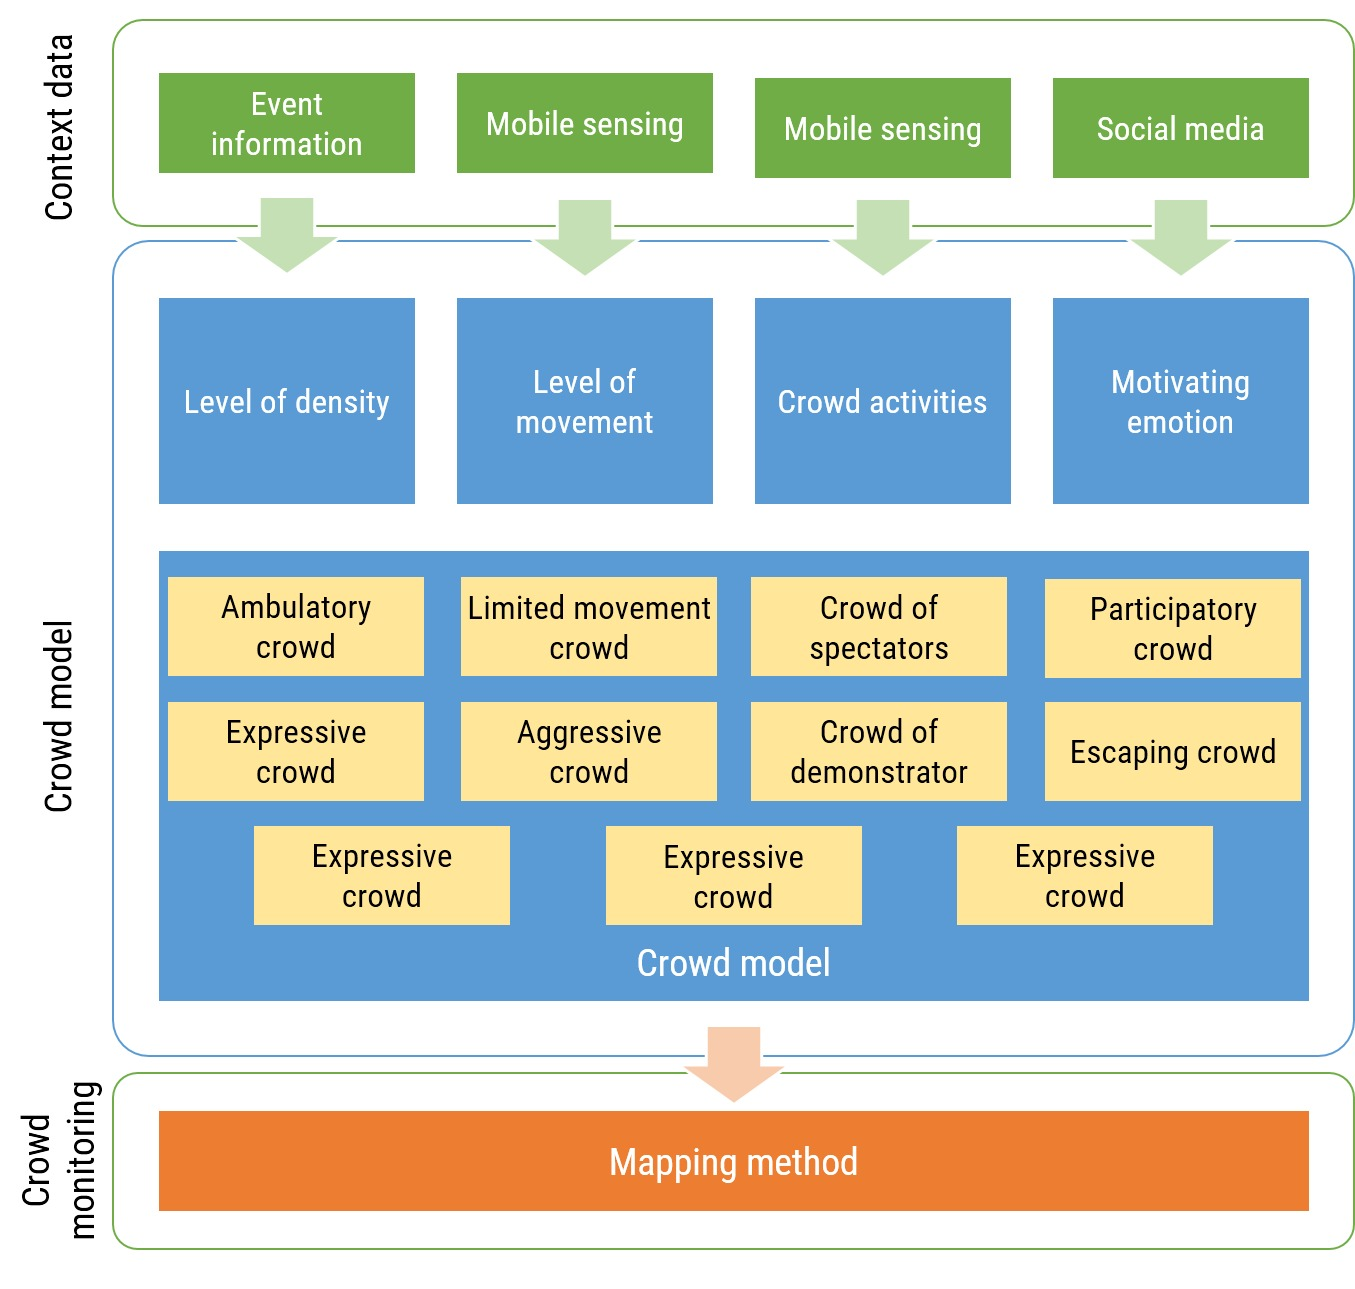
\includegraphics[width=1.0\textwidth]{FrameworkOverview}
	\caption{Overview of the Mobile Crowd Monitoring for Emergency Management in Mass Gathering}
	\label{fig:frameworkOverview}
\end{figure}

Each component will be discussed further in the sections below.

\section{Context Data}

As concluded in Chapter \ref{ch:litReview}, with the rapid development of mobile devices and mobile computing, the literature review has showed the potential of combining different information sources, such as mobile sensors and social media, in a crowd monitoring approach. In our framework, the context data layer is designed to fulfill this objective and serves as the input for the other layers down the stack.

The context data layer collects information about the context, which is the mass gathering event. In the development of a domain ontology for mass gathering, \citet{DelirHaghighi2013a} has summarised a set of related features that might have the effect on the safety of an event, such as environmental factors, event type, crowd size and venue. These knowledge can be retrieved from different sources. For this crowd monitoring framework, we propose three main sources: 
\begin{inparaenum}[i)]
	\item event information;
	\item mobile sensing;
	\item social media
\end{inparaenum}, each of which will be discussed in detail in the following sections.

\subsection{Event Information}
Event information includes information about the venue, expected number of participants or crowd size, and the type of event. This information is static and not required to be collected in real time, hence it can be prepared in the pre-event phase of the emergency management. Ideally, it can be either crawled from the events' homepages or provided by the event organizers and gathered at a centralized system for the monitoring phase.

One of the important features of a mass gathering in the context of emergency management is crowd density, which is the key factor leading to trampling and crushing incidents \citet{Hughes2009}. This information can be estimated by using collected data above, namely the estimated crowd size, the venue capacity and the size of venue following below formula.

\[
crowd\_density = crowd\_size / venue\_size
\]
where, \(crowd\_density\) is the estimated crowd density, \(crowd\_size\) is the number of participants or the venue capacity and \(venue\_size\) is the area of the venue holding the event.

\subsection{Mobile Sensing}

Mobile sensing paradigm has become an emerging topic among recent studies in mobile and context aware computing. It leverages the power of sensor-enhanced mobile devices to acquire information about the context \citep{guo2014participatory}. The mobile devices include modern smart-phones and devices, which are integrated with a wide range of sensors such as GPS receivers, accelerometers and ambient light sensors.

Using the built-in GPS receiver in mobile phones to collect information for crowd monitoring has been proposed in a related works proposed by \citet{Wirz2012}. As mentioned in the literature review, in this study, GPS is used to obtain the current location of the phone bearer. The continuous sampling of the location can be used to estimate the movement of the crowd and the crowd density.

Another integrated sensor in mobile phones that can be used to gather context data is the accelerometer. Accelerometer is often used for the purpose of activity recognition \citep{ravi2005activity, kwapisz2011activity}. In our context of crowd monitoring, the literature review has noted a related work from \citet{Roggen2011}, where several crowd activities can be determined by analysing the pattern of accelerometer's data.

Interestingly, the microphone in mobile phones can also act as a sensor to count the number of devices in a crowd \citep{Kannan2012, Xu2013}, thus can be eventually used to roughly estimate the number of participants. Table \ref{table:mobileSensingCrowdFeature} summarises the possible sensing sources that can be integrated into our framework and the knowledge about a crowd that can be inferred from these sensors.

\begin{table}
	\caption{Mobile sensors and Crowd features}
	\label{table:mobileSensingCrowdFeature}
	\centering
	\begin{tabular}{|l|l|}
		\hline
		\textbf{Mobile sensor} & \textbf{Crowd features} \\
		\hline
		GPS receiver & Movement and density \\
		\hline
		Accelerometer & Activity \\
		\hline
		Microphone & Density \\
		\hline
	\end{tabular}
\end{table}

The role of mobile sensing in our crowd monitoring framework is to provide the real-time data about a mass gathering event. As mentioned in the previous chapter, the during event phase in emergency management requires real-time decision making, which requires continuously updated intelligence from the crowd monitoring system. The reason for this requirement is that, according to \citet{Berlonghi1995}, a particular crowd can change from one type to another type during the event. This dynamic nature of a crowd is the key factor that we want to address in our approach by integrating the mobile sensing as one of the sources of context data.

\subsection{Social Media}

Social media is another source of information that is capable of providing real-time data. In a related work, social media is considered as a special ``soft sensor'' in the mobile sensing techniques used in crowd monitoring \citep{Ramesh2014}. Social media is a generic term referring to a wide range of Internet-based tools that enable users to create and share content. It might include social network sites, such as Twitter and Facebook, Internet forums and channels.

\section{Crowd Model}

As mentioned in the literature review, there has been a very limited work on crowd modelling. Berlonghi's model is among the most widely adopted by emergency management bureaus worldwide. 

\subsection{Comparison of different Crowd Models}

\begin{center}
	\begin{longtable}{|p{2.2cm}|p{2cm}|p{2cm}|p{4.2cm}|p{2.8cm}|}
	\caption{Comparison of different Crowd Models}
	\label{table:crowdModelComparison} \\
	\hline
	\multirow{2}{\linewidth}{\textbf{Crowd type}} & \multicolumn{3}{c|}{\textbf{Origin}} & \multirow{2}{\linewidth}{\textbf{Example}} \\
	\cline{2-4}
	& Crowd type & Source & Definition & \\
	
	\hline
	\multirow{2}{\linewidth}{Ambulatory crowd} & Ambulatory \newline \newline & \citet{Berlonghi1995} & \multirow{2}{\linewidth}{People are walking in and out or to and from a venue \citep{Berlonghi1995}. Usually characterized by the calm movement \citep{Zeitz2009}} & \multirow{2}{\linewidth}{People entering a stadium or a concert} \\
	\cline{2-3}
	& Casual crowd \newline & \citet{Blumer1951} & & \\

	\hline
	\multirow{2}{\linewidth}{Limited movement crowd} & Disability / Limited movement \newline \newline & \citet{Berlonghi1995} & \multirow{2}{\linewidth}{People are limited or restricted in movement \citep{Berlonghi1995}. People have loose connection and little interaction \citep{Blumer1951}. People happen to be at a given place but not unified or organized \citep{Momboisse1967}} & \multirow{2}{\linewidth}{People waiting in a queue to get tickets} \\
	\cline{2-3}
	& Casual crowd \newline \newline \newline & \citet{Blumer1951} & & \\

	\hline
	\multirow{2}{\linewidth}{Crowd of spectators} & Cohesive / Spectators \newline \newline \newline & \citet{Berlonghi1995} & \multirow{2}{\linewidth}{People are present to watch a specific event, not to communicate with each other. Characterized by the desire to stay and watch \citep{Berlonghi1995}. People are assembled for a specific purpose \citep{Blumer1951}} & \multirow{2}{\linewidth}{People watching a football game in the stadium or catching a concert in a theatre} \\
	\cline{2-3}
	& Conventional crowd \newline \newline \newline & \citet{Blumer1951} & & \\

	\hline
	\multirow{2}{\linewidth}{Participatory crowd} & Participatory & \citet{Berlonghi1995} & \multirow{2}{\linewidth}{People are involved in actual activities of an event \citep{Berlonghi1995}} & \multirow{2}{\linewidth}{People walking in a parade} \\
	\cline{2-3}
	& Conventional crowd & \citet{Blumer1951} & & \\

	\hline
	\multirow{3}{\linewidth}{Expressive crowd} & Expressive / revellous & \citet{Berlonghi1995} & \multirow{3}{\linewidth}{People are involved in an emotional release \citep{Berlonghi1995}} & \multirow{3}{\linewidth}{People cheering, chanting in unison. Human wave in a soccer match} \\
	\cline{2-3}
	& Expressive crowd & \citet{Blumer1951} & & \\
	\cline{2-3}	
	& Expressive crowd & \citet{Momboisse1967} & & \\	

	\hline
	\multirow{2}{\linewidth}{Aggressive crowd} & Aggressive / Hostile & \citet{Berlonghi1995} & \multirow{2}{\linewidth}{People are verbally assaultive and showing disregard \citep{Berlonghi1995}} & \multirow{2}{\linewidth}{Soccer hooligan shouting} \\
	\cline{2-3}
	& Hostile or aggressive crowd & \citet{Momboisse1967} & & \\

	\hline
	\multirow{2}{\linewidth}{Crowd of demonstrators} & Demonstrator \newline \newline & \citet{Berlonghi1995} & \multirow{2}{\linewidth}{People are organized by an established leadership for specific reason \citep{Berlonghi1995}. A crowd which has some political goal \citep{Imhonopi2013}} & \multirow{2}{\linewidth}{A protest, a picket} \\
	\cline{2-3}
	& Protest crowd & \citet{McPhail1983} & & \\

	\hline
	\multirow{4}{\linewidth}{Escaping crowd} & Escaping / Trampling & \citet{Berlonghi1995} & \multirow{4}{\linewidth}{People are trying to escape from a danger or a threat \citep{Berlonghi1995, Momboisse1967}} & \multirow{4}{\linewidth}{A evacuation from a fire} \\
	\cline{2-3}
	& Escapist mob & \citet{Blumer1951} & & \\
	\cline{2-3}	
	& Trampling & \citet{Hughes2009} & & \\
	\cline{2-3}
	& Acting crowd & \citet{Blumer1951} & & \\

	\hline
	\multirow{2}{\linewidth}{Crushing crowd} & Dense / Suffocating \newline \newline & \citet{Berlonghi1995} & \multirow{2}{\linewidth}{People have limited individual movement \citep{Berlonghi1995} and being compressed. Characterized by high density \citep{Lee2005}} & \multirow{2}{\linewidth}{A human stampede at new year festival} \\
	\cline{2-3}
	& Crushing & \citet{Lee2005} & & \\

	\hline
	\multirow{3}{\linewidth}{Expressive crowd} & Rushing / looting & \citet{Berlonghi1995} & \multirow{3}{\linewidth}{People are trying to obtain or steal something \citep{Berlonghi1995}} & \multirow{3}{\linewidth}{People looting food after a natural disaster} \\
	\cline{2-3}
	& Acquisitive mob & \citet{Momboisse1967} & & \\
	\cline{2-3}	
	& Acting crowd & \citet{Blumer1951} & & \\	

	\hline
	\multirow{3}{\linewidth}{Violent crowd} & Violent & \citet{Berlonghi1995} & \multirow{3}{\linewidth}{People are attacking and rioting with disregard for laws and rights \citep{Berlonghi1995}} & \multirow{3}{\linewidth}{A riot in Ferguson, USA} \\
	\cline{2-3}
	& Aggressive mob & \citet{Momboisse1967} & & \\
	\cline{2-3}	
	& Acting crowd & \citet{Blumer1951} & & \\	

	\hline
	\end{longtable}
\end{center}

\subsection{Crowd Types}

\begin{itemize}
	\item Ambulatory crowd
	\item Limited movement crowd
	\item Crowd of spectators
	\item Participatory crowd
	\item Expressive crowd
	\item Aggressive crowd
	\item Crowd of demonstrator
	\item Escaping crowd
	\item Looting crowd
	\item Rushing crowd
	\item Violent crowd
\end{itemize}

\subsection{Crowd Attributes}

\begin{itemize}
	\item Level of Density
	\item Level of Movement
	\item Crowd Activities
	\item Motivating Emotions
\end{itemize}

\section{Crowd Monitoring}


%\subsection{Emotion in the crowd}

%\section{Crowd Monitoring using Emotion Analysis of Social Media}

%\subsection{Social Media Analysis}

%\subsubsection{Twitter as the Context data}

%\subsubsection{Twitter Analysis}

%\subsection{Emotion Analysis}

%\subsubsection{The Word-Emotion Lexicon}

%\subsubsection{The use of Voting System for Emotion Classification}

%\subsection{Realtime Crowd Monitoring}

%\subsubsection{Mapping emotion into crowd types}

%\subsubsection{Realtime detection of dangerous crowd types}

\section{Conclusion}